\documentclass{report} 
\title{Appendix 2}
\date{Started 24 May 2024}
\author{Malcolm}
\usepackage{amsmath} %import math
\usepackage{mathtools} %more math
\usepackage{amssymb} %for QED symbol
\usepackage{amsthm} %
\usepackage{bm}%bold math
\usepackage{graphicx} %import imaging
\graphicspath{{./images/}} %set imaging path
\begin{document}
\maketitle

\tableofcontents

\appendix
\chapter{Differential Equations}
\section{Fundamentals}
\subsection{Introduction to Ordinary Differential Equations\\(ODEs)} %030624
Here we introduce intuition for  Ordinary Differential Equations (ODEs) and introductory solving methods.\\
\vspace{1mm}\\
The simplest type of differential equation looks like:
\begin{equation*}
\frac{dy}{dx}=f(x)
\end{equation*}
which can be solved by the antiderivative $y=\int f(x)\,dx$. \\
\vspace{1mm}\\
\textbf{Intuition}\\
Now we consider a more interesting example: 
\begin{equation*}
\frac{dy}{dx}+xy=0
\end{equation*}
This equation can be solved by \textit{separation of variables}:
\begin{align*}
\frac{dy}{dx}+xy&=0\\
\frac{dy}{dx}&=-xy\\
\frac{dy}{y}&=-x\,dx
\end{align*}\\
(next page)\\
Since the problem is now set up in terms of differentials rather than ratios of differentials,
we can integrate both sides.
\begin{align*}
\int\frac{dy}{y}&=-\int x\,dx\\
\ln y+c_1&=-\frac{x^2}{2}+c_2\quad\text{(assume $y>0$)}
\end{align*}
We can combine the constants and simplify:
\begin{align*}
\ln y&=-\frac{x^2}{2}+c\\
e^{\ln y}&=e^{-x^2/2+c}\\
y&=e^ce^{-x^2/2}\\
y&=Ae^{-x^2/2},\quad\text{(where $A=e^c$})
\end{align*}
(The more apt $\ln|y|$ simplifies to $\pm Ae^{-x^2/2}$, which doesn't matter since $A$ is some
unspecific constant)\\
\vspace{1mm}\\
It turns out that our solution,
\begin{equation*}
y=Ae^{-x^2/2},\quad\text{(where $A=e^c$})
\end{equation*}
Works for any constant multiple $A$. We can check this 
solution:
\begin{align*}
y&=ae^{-x^2/2}\\
\frac{dy}{dx}&=\frac{d}{dx}ae^{-x^2/2}\\
&=a\cdot(-x)e^{-x^2/2}\\
&=-x\cdot ae^{-x^2/2}\\
\frac{dy}{dx}&=-xy
\end{align*}
$A$ is determined by an initial condition; for instance if $y(0)=1$, $A=1$.
\newpage

\subsection{Separation of Variables} %030524
Here we describe a rudimentary method for solving some differential equations---\\Separation of Variables.\\
\vspace{1mm}\\
In general, this method applies to differential equations of the form
\begin{equation*}
\frac{dy}{dx}=f(x)g(y)
\end{equation*}
Where we then \textit{separate} the variables and integrate:
\begin{align*}
\frac{dy}{dx}&=f(x)g(y)\\
\frac{dy}{g(y)}&=f(x)\,dx\\
h(y)\,dy&=f(x)\,dx\quad\text{where }h(y)=\frac{1}{g(y)}\\
\int h(y)\,dy&=\int f(x)\,dx\\
\end{align*}
Antidifferentiating both sides:
\begin{equation*}
H(y)=\int h(y)\,dy;\quad F(x)=\int f(x)\,dx
\end{equation*}
we now have
\begin{align*}
H(y)+c_1&=F(x)+c_2\\
H(y)&=F(x)+c
\end{align*}
\newpage

\subsection{Direction fields, Isoclines, and Integral curves}%131024
\textbf{Direction fields}\\
Given an equation $y'=f(x,y)$, we can construct a \textit{direction field}; imagine through each point $(x,y)$, we
draw a line segment whose slope is $f(x,y)$---consider $y'(x)=2x$:
\begin{figure}[h]
\begin{center}
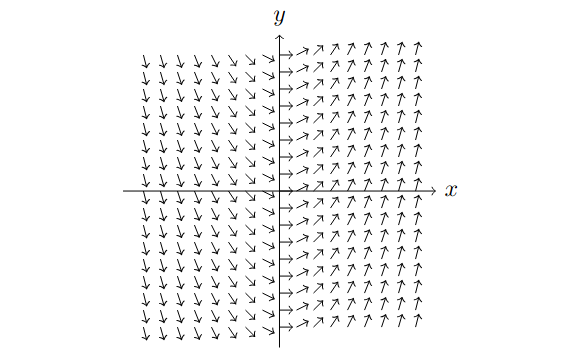
\includegraphics[width=10cm]{1}\\
\end{center}
(note that in this case $f(x,y)$ does not depend on $y$ (because of the equation)---it is invariant under vertical
translation)
\end{figure}\\
\textbf{Plotting direction fields---Isoclines}\\
In practice, computers are used to plot direction fields following the procedure:
\begin{enumerate}
\item Pick point $(x,y)$
\item Compute $y'=f(x,y)$
\item Plot line segment of slope at that point
\end{enumerate}
Notice how a new slope has to be computed for each specified point; when plotting direction fields by hand, 
it is much more practical to utilise \textit{isoclines}, which are, given the equation $y'=f(x,y)$, a one-parameter
family of curves given by the equations
\begin{equation*}
f(x,y)=m,\quad m\text{ constant}
\end{equation*}
Along a given isocline, all line segments have the same slope $m$.\\
(next page)
\newpage
\noindent\textbf{Example}\\
Consider plotting the direction field for the equation
$y'=x-y$; the isoclines are correspondingly the lines
$x-y=m$ (shown in dashed lines):
\begin{figure}[h]
\begin{center}
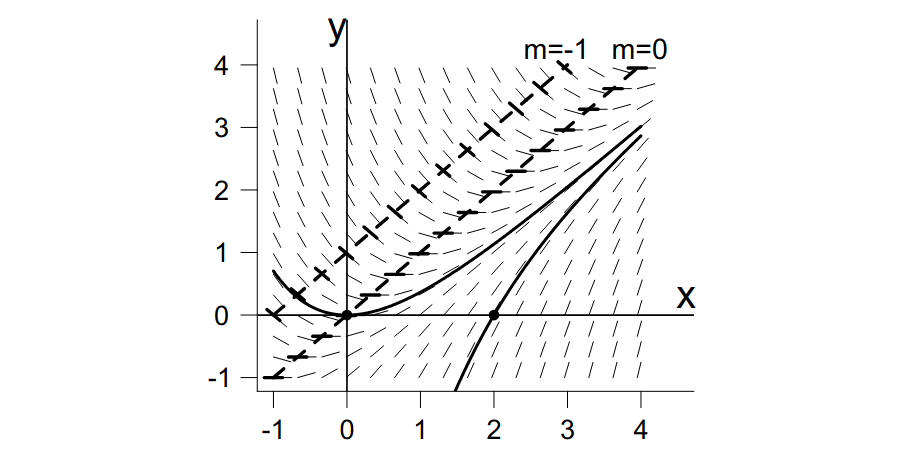
\includegraphics[width=10cm]{2}\\
\end{center}
The $m=0$ isocline marks the points where the slope of the solution is 0; it is therefore of special interest 
and is called the \textit{nullcline}.
\end{figure}\\
\textbf{Integral curves}\\
As also shown in the figure above, once the direction field has been sketched, curves which are \textit{at each
point tangent to the line segment at that point} can be drawn; 
such curves are called \textit{integral curves} or \textit{solution curves} for the direction field.
Their significance (this should be obvious) is that
\begin{equation*}
\text{\textit{The integral curves are the graphs of the solutions to }}y'=f(x,y)
\end{equation*}
Two integral curves have been drawn above (in solid lines).\\
\vspace{1mm}\\
\textbf{Intersection Principle}\\
Intuitively, see that at any point in the direction field it can only have one direction; therefore it is fairly
obvious that integral curves cannot cross at an angle.\\
\vspace{1mm}\\
Consider the existence and uniqueness theorem for ODEs: 
\begin{align*}
&\text{\textit{For any $(a,b)$ in the region where $f$ is defined, $y'=f(x,y)$ has}}\\&\text{\textit{exactly one solution such that 
$y(a)=b$.}}
\end{align*}
by the existence part of the theorem, 
there is an integral curve through any point where $f(x,y)$ is defined. Now supposing two integral curves
through the same point, by the uniqueness part of the theorem they must agree.\\
\vspace{1mm}\\
As a result, \textit{integral curves cannot intersect}; every point lies on exactly one integral curve.
\newpage

\subsection{Long term Behaviour: Fences, Funnels, and Separatrices}%140824
\textbf{Fences}\\
A \textit{lower fence} for the equation $y'=f(x,y)$ is a curve that `blocks' an integral curve from crossing from
\textit{above}; intuitively it is the curve whose direction field elements along the curve point up from it. Technically 
it can be described as a curve $y=L(x)$ such that $L'(x)<f(x,L(x))$ (the slope of the curve is always 
less than the slope of the direction field at that point).\\
\vspace{1mm}\\
Likewise an \textit{upper fence} is a curve that `blocks' integral curves from crossing from \textit{above}. 
Illustrated:
\begin{figure}[h]
\begin{center}
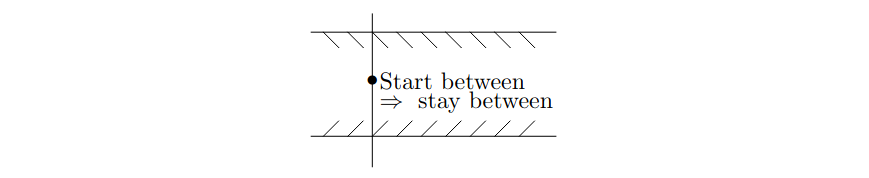
\includegraphics[width=10cm]{3}\\
\end{center}
(The upper curve is the upper fence and the lower curve is the lower fence). Solutions will be `squeezed' between
upper and lower fences.
\end{figure}\\
Note that
\begin{itemize}
\item Note that fences aren't necessarily defined for all $x$; they could be defined only on an interval like
$x\geq c$ for some constant $c$.
\item Since integral curves can't cross an integral curve itself it is both an upper and lower fence.
\end{itemize}
(next page)
\newpage
\noindent\textbf{Example}\\
Consider the direction field for the equation
\begin{equation*}
y'=y^2-x
\end{equation*}
The isoclines for $m=0$ and $m=-1$ are plotted in yellow, with integral curves in blue:
\begin{figure}[h]
\begin{center}
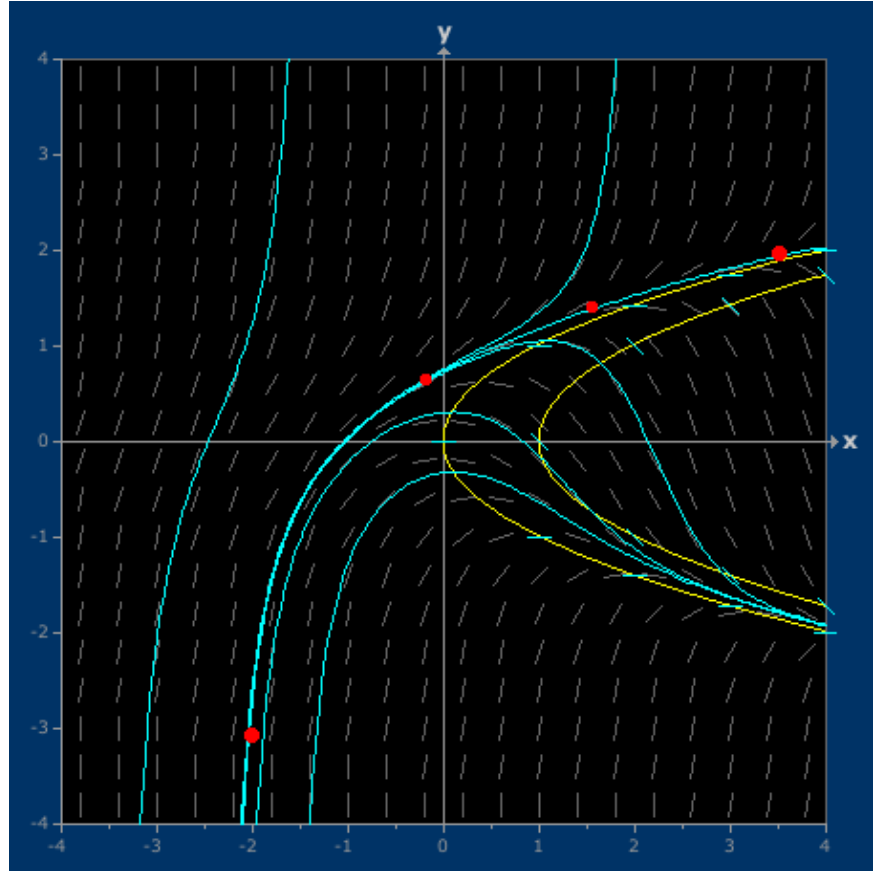
\includegraphics[width=10cm]{4}\\
\end{center}
Notice that the bottom hald of the isocline $m=0$ is a lower fence and for $x$ large enough the bottom 
half of the isocline $m=-1$ is an upper fence. (notice that the $m=-1$ isocline becomes an upper
fence only for $x$ large enough)
\end{figure}\\
(next page)
\newpage
\noindent\textbf{Funnels}\\
One use of fences is to construct funnels. A \textit{funnel} for the equation $y'=f(x,y)$ consists of a pair of 
fences; one lower fence $L(x)$ and one upper fence $U(x)$ with the properties
\begin{enumerate}
\item For $x$ large the lower fence is below the upper fence; $L(x)<U(x)$
\item The two fences come together asymptotically; $U(x)-L(x)$ is small for large $x$
\end{enumerate}
For instance, in the above example the bottom parts of the two isoclines $m=0$ and $m=-1$ act as a funnel
once $x$ is large enough. Given the equations of each isocline we have highly accurate estimates for solutions
between them as
\begin{equation*}
\underbrace{-\sqrt{x}}_{m=0}<y(x)<\underbrace{-\sqrt{x-1}}_{m=-1}
\end{equation*}
which is valid for large $x$.\\
\vspace{1mm}\\
Note that not all pairs of upper/lower fences form a funnel---they have to come together asymptotically as $x$ 
gets large.\\
\vspace{1mm}\\
\textbf{Separatrices}\\
A \textit{separatrix} is an integral curve such that the integral curves above it behave entirely differently from
integral curves below it as $x\to\infty$.
\newpage

\subsection{Runge-Kutta 2 (Numerical methods)}%161024
\textbf{General approach and Euler's method}\\
Euler's method (for numerical estimation) follows a more general procedure for stepping from 
$(x_n,y_n)$ to $(x_{n+1},y_{n+1})$:
\begin{equation*}
x_{n+1}=x_n+h,\quad y_{n+1}=y_n+m_nh
\end{equation*}
Where $h$ is the stepsize in the $x$ direction and $m$ is the slope of the line we step along. In Euler's
method $h$ is fixed ahead of time and $m_n=f(x_n,y_n)$.\\
\vspace{1mm}\\
\textbf{Runge-Kutta 2}\\
Naturally Euler's method is a fairly flawed method of numerical estimation. Other methods use other (and better)
ways of choosing $h$ and $m$. Here I describe the \textit{Runge-Kutta 2} (RK2) method, which is a
\textit{fixed stepsize} method; meaning $h$ is fixed and the added complexity comes from finding $m$.\\
\vspace{1mm}\\
Given an initial value problem $y'=f(x,y),y(x_0)=x_0$ and a step size $h$, one step of the RK2 method is as follows:
\begin{enumerate}
\item Compute the slope $k_1$ at $(x_0,y_0)$: $k_1=f(x_0,y_0)$
\item `Take' an Euler step from $(x_0,y_0)$ to $(a,b):$ $a=x_0+h,$  $b=y_0+k_1h$
\item Compute the slope $k_2$ at $(a,b):$ $k_2=f(a,b)$
\item Average $k_1$ and $k_2$ to get $m$: $m=(k_1+k_2)/2$
\item Now we use this averaged slope to take a step from 
$(x_n,y_n)$ to $(x_{n+1},y_{n+1})$: 
\begin{equation*}
x_{1}=x_0+h,\quad y_{1}=y_0+mh;\quad m=\frac{(k_1+k_2)}{2}
\end{equation*}
\end{enumerate}
Other methods such as RK4 or \textit{variable stepsize methods} may (probably) work better. Though one might want
to consider computational efficiency at the expense of accuracy.
\newpage

\subsection{First order Linear Differential Equations}%181024
\textbf{Definition}\\
The general \textit{First order linear ODE} in the unknown function $x=x(t)$ has the form
\begin{equation*}
A(t)\frac{dx}{dt}+B(t)x(t)=C(t)
\end{equation*}
If $A(t)\neq0$ we can simplify the equation by dividing by $A(t)$:
\begin{equation*}
\frac{dx}{dt}+p(t)x(t)=q(t)
\end{equation*}
This is called the \textit{standard form} for a first order linear ODE. Should the \textit{coefficients} $A(t),B(t)$
be constants (not dependent on $t$) we say the equation is a \textit{constant coefficient} DE.\\
\vspace{1mm}\\
If $C(t)=0$:
\begin{equation*}
A(t)\frac{dx}{dt}+B(t)x(t)=0
\end{equation*}
The DE is called \textit{homogeneous} (notice that conversion to standard form doesn't change this fact); otherwise
the equation is \textit{inhomogeneous}.\\
\vspace{1mm}\\
\textbf{Signals and Systems---Terminology}\\
Given a differential equation
\begin{equation*}
\frac{dx}{dt}+p(t)x(t)=q(t)
\end{equation*}
Notice that the right-hand side does not depend on $x$. The left-hand side represents the \textit{system}
(think of it as defining the behaviour of a system); the
right-hand side represents an outside influence on the system, which we can call the \textit{input}.\\
\vspace{1mm}\\
In general, a signal is a function of $t$. The system \textit{responds} to the input signal and yields
the function $x(t)$, which we call the \textit{output signal} or \textit{system response}. (these terms should just
be seen as convenient convention when describing an ODE)\\
\vspace{1mm}\\
\textit{Block diagrams} can be used to visually represent systems:
\begin{figure}[h]
\begin{center}
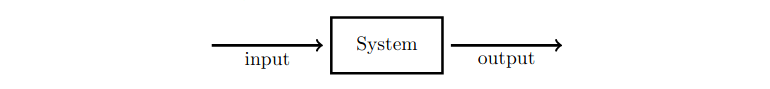
\includegraphics[width=10cm]{5}\\
\end{center}
(next page)
\end{figure}
\newpage
\noindent\textbf{Example---RC circuits}\\
Suppose we have an electrical circuit as shown
\begin{figure}[h]
\begin{center}
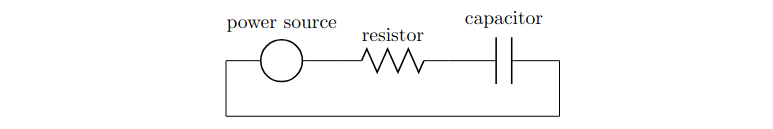
\includegraphics[width=10cm]{6}\\
\end{center}
``Kirchhoff's Voltage Law'' states that the total voltage change around the loop is 0, meaning
\begin{equation*}
V(t)=V_R(t)+V_C(t)
\end{equation*}
The relationship between voltage drop and current are described as follows:
\begin{align*}
&\text{Resistor: }V_R(t)=RI(t)\text{ for a constant }R,\text{ the ``resistance''}\\
&\text{Capacitor: }V'_C(t)=\frac{1}{C}I(t)\text{ for a constant }C,\text{ the ``capacitance''}
\end{align*}
the voltage drop from the capacitance can be seen from
the equation defining capacitance
\begin{align*}
q&=CV\quad\text{(charge per unit voltage)}\\
I(t)=\frac{dq}{dt}&=\frac{d}{dt}(CV)\\
I(t)&=CV'\quad\text{($C$ constant)}\\
V'_C(t)&=\frac{1}{C}I(t)
\end{align*}
The voltage drop across the capacitor is proportional to the \textit{integral} of the current; it results from
a buildup of charge on two plates of the capacitor.\\
(next page)
\end{figure}
\newpage
\noindent We can differentiate Kirchhoff's Voltage Law 
\begin{align*}
V'(t)&=V_R'(t)+V_C'(t)\\
&=RI'(t)+\frac{1}{C}I(t)
\end{align*}
to obtain a first order linear differential equation
\begin{equation*}
RI'(t)+\frac{1}{C}I(t)=V'(t)
\end{equation*}
In this circuit we consider the voltage $V(t)$ to be the input signal, and the circuit with resistance $R$ and
capacitance $C$ to be the system. The current $I$ is the output signal/system response:
\begin{figure}[h]
\begin{center}
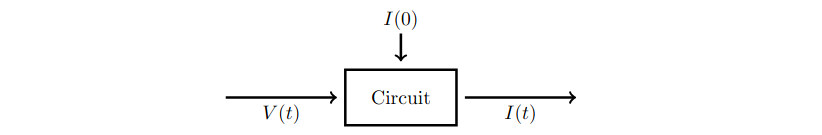
\includegraphics[width=10cm]{7}\\
\end{center}
$I(0)$ represents the initial condition.
\end{figure}
\newpage

\subsection{Superposition (First order ODEs)}%191024
Considering the following the first order linear equation:
\begin{equation*}
\dot{y}+p(t)y=q(t)
\end{equation*}
If a given input $q(t)$ has the output $y(t)$ we write
\begin{equation*}
q\rightsquigarrow y
\end{equation*}
Here we show that if
\begin{equation*}
q_1\rightsquigarrow y_1\text{ and }q_2\rightsquigarrow y_2
\quad\text{then}\quad c_1q_1+c_2q_2\rightsquigarrow
c_1y_1+c_2y_2
\end{equation*}
\textbf{Proof}\\
First see that (since differentiation does't change the constant coefficient)
\begin{align*}
\frac{dy}{dt}+py&=q\\
c\frac{dy}{dt}+cpy&=cq\\
=\frac{d(cy)}{dt}+p(cy)&=cq;\quad cq\rightsquigarrow cy
\end{align*}
Now see that
\begin{align*}
\frac{d(c_1y_1+c_2y_2)}{dt}+p(c_1y_1+c_2y_2)
&=\underbrace{c_1\dot{y}_1+pc_1y_1}_{=c_1q_1}
+\underbrace{c_2\dot{y}_2+pc_2y_2}_{=c_2q_2}\\
&=c_1q_1+c_2q_2
\end{align*}
Essentially, any linear combination of solutions is also a solution.
\newpage

\subsection{Solution by Integrating Factor (inhomogenous first order ODEs)}%240824
Here we prove the general solution to the inhomogeneous first order linear ODE 
\begin{equation*}
\dot{x}+p(t)x=q(t)
\end{equation*}
is\begin{equation*}
x(t)=\frac{1}{u(t)}\left(\int u(t)q(t)dt+C\right),
\quad\text{where }u(t)=e^{\int p(t)dt}
\end{equation*}
the function $u$ is called an \textit{integrating factor}.\\\vspace{1mm}\\
\textbf{Proof}\\
We start with the product rule for differentiation:
\begin{equation*}
\frac{d}{dt}(ux)=u\dot{x}+\dot{u}x
\end{equation*}
Consider multiplying both sides of our inhomogenous first order ODE by some function $u(t)$:
\begin{equation*}
u\dot{x}+upx=uq
\end{equation*}
We want to choose a function $u(t)$ such that we can apply the product rule to the sum on the left hand side
of the equation. There may be many functions $u$ that could work, but in this case we only need one. See that
\begin{equation*}
\frac{d}{dt}(ux)=u\dot{x}+\dot{u}x\iff u\dot{x}+upx=u\dot{x}+\dot{u}x\iff
\dot{u}=up
\end{equation*}
so now by separation of equations
\begin{align*}
\frac{du}{u}&=p(t)dt\\
\ln|u|&=\int p(t)dt\\
u&=e^{\int p\,dt}
\end{align*}
By using $u$ to satisfy the product rule:
\begin{align*}
u\dot{x}+upx=\frac{d}{dt}(ux)&=uq\\
u(t)x(t)&=\int u(t)q(t)dt+c\\
x(t)&=\frac{1}{u(t)}\left(\int u(t)q(t)dt+c\right)
\end{align*}
which was what we wanted.\\
(next page)
\newpage
\noindent\textbf{Integrating factor and homogeneous equations}\\
Given the homogeneous first order ODE
\begin{equation*}
\dot{x}+p(t)x=0
\end{equation*}
Solving by separation of variables gives
\begin{equation*}
x_h(t)=Ae^{-\int p(t)dt}
\end{equation*}
Comparing this to the formula for the integrating factor
\begin{equation*}
u(t)=e^{\int p(t)dt}
\end{equation*}
see that
\begin{equation*}
x_h(t)=\frac{A}{u(t)}
\end{equation*}
\newpage

\subsection{General, Particular and Homogeneous solutions}%301024
Solving by method of Integrating factors allows us to come up with a solution for inhomogeneous first order linear
ODEs
\begin{equation*}
\dot{x}+p(t)x=q(t)
\end{equation*}
Which have the form
\begin{equation*}
x(t)=\frac{1}{u(t)}\left(\int u(t)q(t)dt+C\right),
\quad\text{where }u(t)=e^{\int p(t)dt}
\end{equation*}
Notice that the presence of the constant $C$ implies a family of solutions; by setting $C=0$ we get a
\textit{particular solution} $x_p$, which is simply one specific solution---we could have chosen any other:
\begin{align*}
x_p=\frac{1}{u(t)}\left(\int u(t)q(t)dt+0\right)\quad&\text{is a solution}\\
x_p=\frac{1}{u(t)}\left(\int u(t)q(t)dt+999\right)\quad&\text{is also a solution}
\end{align*}
The method of integrating factors naturally leaves us with a constant. But say we were to find a solution by 
\textit{inspection}---how would we know that the constant of integration exists in the form $\frac{C}{u(t)}$? (as
is in this case)\\
\vspace{1mm}\\
\textbf{General solution}\\
See that since
\begin{equation*}
x_h(t)=\frac{1}{u(t)}
\end{equation*}
We can write the solution by integrating factor as
\begin{align*}
x(t)&=\frac{1}{u(t)}\left(\int u(t)q(t)dt\right)+\frac{C}{u(t)}\\
&=x_p+Cx_h
\end{align*}
One way to fully solve the inhomogeneous equation is by first solving the \textit{homogeneous} equation, and
then finding any \textit{one} solution, a \textit{particular solution}, to the inhomogeneous equation $x_p$. 
(We can use any method to find $x_p$ since we the homogeneous solution handles the constant of integration):
\begin{equation*}
\text{General solution}=\text{Particular solution}+\text{Homogeneous solution}
\end{equation*}
(next page)
\newpage
\noindent\textbf{Intuition}\\
Given an inhomogeneous first order linear ODE and its associated homogeneous equation
\begin{align*}
\dot{x}+p(t)x=q(t)\quad&\text{(inhomogeneous)}\\
\dot{x}+p(t)x=0\quad&\text{(homogeneous)}
\end{align*}
Solving both equations by method of integrating factors gives
\begin{equation*}
x_p(t)=\frac{1}{u(t)}\left(\int u(t)q(t)dt\right)+\frac{A}{u(t)},\qquad
x_h(t)=\frac{B}{u(t)}
\end{equation*}
(where $A$ is any chosen constant, each constant giving a particular solution, and $B$ the constant of integration)
Now see that by adding the solutions together the constant for the inhomogeneous solution $A$ gets absorbed into
the homogeneous solution:
\begin{align*}
x_p(t)+x_h(t)&=\frac{1}{u(t)}\left(\int u(t)q(t)dt\right)+\frac{A+B}{u(t)}\\
&=\frac{1}{u(t)}\left(\int u(t)q(t)dt\right)+\frac{C}{u(t)}
\end{align*}
We can obtain the `ambiguous part' of the general solution by simply solving the homogeneous equation; this means
that when obtaining a particular solution we don't have to worry about the constant of integration.\\
\vspace{1mm}\\
\textbf{Superposition}\\
See that this also makes sense with respect to superposition of solutions, where since
\begin{equation*}
\underbrace{q(t)\rightsquigarrow x_p(t)}_{\text{inhomogeneous}}\quad\text{and}\quad
\underbrace{0\rightsquigarrow x_h(t)}_{\text{homogeneous}}
\end{equation*}
we can say
\begin{equation*}
q(t)+0=q(t)\rightsquigarrow x_p(t)+x_h(t)
\end{equation*}
\newpage

\subsection{Polar form and Euler Identity}%311024
\textbf{The Complex Plane, Polar Form}\\
Complex numbers can be represented geometrically by points in a plane, where the number $a+ib$ is represented by 
the point $(a,b)$; when points in a plane are thought of as representing complex numbers this way,
the plane is known as a \textit{Complex Plane}:
\begin{figure}[h]
\begin{center}
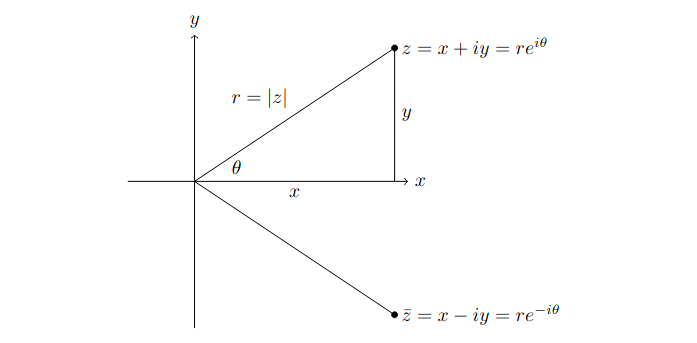
\includegraphics[width=9cm]{8}\\
\end{center}
See that the magnitude of the coordinates of a complex number $x+iy$ can be represented by
\begin{equation*}
x=r\cos(\theta),\quad y=r\sin(\theta)
\end{equation*}
where $r$ is the absolute value of the number:
\begin{equation*}
r=|x+iy|=\sqrt{x^2+y^2}
\end{equation*}
(its just the pythagorean theorem) thus the entire number
can be written as
\begin{equation*}
x+iy=r(\cos(\theta)+i\sin(\theta))
\end{equation*}
This is called the \textit{Polar Form}
of a non-zero complex number. We call $\theta$ the \textit{angle} or
\textit{argument} of $x+iy$:
\begin{equation*}
\theta=\arg(x+iy)
\end{equation*}
Notice that the angle can be increased by any integer multiple of $2\pi$ and will still represent the same thing. 
To simplify this one can specify the \textit{principal value} of the angle:
\begin{equation*}
0\leq\theta<2\pi
\end{equation*}
this can be indicated by $\text{Arg}(...)$; for instance
\begin{equation*}
\text{Arg}(-1)=\pi,\quad\arg(-1)=\pm\pi,\pm3\pi,\pm5\pi
\end{equation*}
\end{figure}\\
(next page)
\newpage
\noindent\textbf{Euler's Formula}\\
Complex numbers have another \textit{exponential} form called \textit{Euler's formula}:
\begin{equation*}
e^{i\theta}=\cos(\theta)+i\sin(\theta)
\end{equation*}
This should be regarded as a definition for the exponential of an imaginary power.\\
\vspace{1mm}\\
A good justification for Euler's formula can be found from
its Taylor approximation:
\begin{align*}
e^{i\theta}&=1+i\theta-\frac{\theta^2}{2!}-i\frac{\theta^3}{3!}+\frac{\theta^4}{4!}+i\frac{\theta^5}{5!}-\cdots\\
&=\left(1-\frac{\theta^2}{2!}+\frac{\theta^4}{4!}-\cdots\right)+i\left(\theta-\frac{\theta^3}{3!}
+\frac{\theta^5}{5!}-\cdots\right)\\
&=\cos(\theta)+i\sin(\theta)
\end{align*}
Note that the argument above is not a proof; rather it just shows that Euler's formula is formally compatible with
the series expansions for the exponential, sine, and cosine functions.\\
\vspace{1mm}\\
\textbf{Polar form again}\\
We can now write
\begin{equation*}
x+iy=r(\cos(\theta)+i\sin(\theta))=re^{i\theta}
\end{equation*}
Polar representation in exponential form allows for much simpler multiplication of complex numbers. Since once can
show that (using angle addition formulas)
\begin{align*}
e^{i\theta_1}e^{i\theta_2}&=(\cos(\theta_1)+i\sin(\theta_1))(\cos(\theta_2)+i\sin(\theta_2))\\
&=\cos(\theta_1)\cos(\theta_2)-\sin(\theta_1)\sin(\theta_2)\\&\quad+i(\sin(\theta_1)\cos(\theta_2)+\cos(\theta_1)\sin(\theta_2)\\
&=\cos(\theta_1+\theta_2)+i\sin(\theta_1+\theta_2)\\
&=e^{i(\theta_1+\theta_2)}
\end{align*}
(next page)
\newpage
\noindent\textbf{Complex Exponential properties}\\
We had
\begin{equation*}
e^{i\theta_1}e^{i\theta_2}=e^{i(\theta_1+\theta_2)}
\end{equation*}
This property can be extrapolated to further justify Euler's formula---the complex exponential follows
the same exponential addition rules as any typical exponential. See that we can now conclude:\\
\vspace{1mm}\\
\textit{Multiplication rule:}
\begin{equation*}
r_1e^{i\theta_1}\cdot r_2e^{i\theta_2}=r_1r_2e^{i(\theta_1+\theta_2)}
\end{equation*}
also see that since
\begin{equation*}
\frac{1}{r}e^{-i\theta}\cdot re^{i\theta}=1
\end{equation*}
\textit{Reciprocal Rule:} 
\begin{equation*}
\frac{1}{re^{i\theta}}=\frac{1}{r}e^{-i\theta}
\end{equation*}
\textbf{DeMoivre's Formula}\\
Since 
\begin{equation*}
(x+iy)^n=r^ne^{in\theta}
\end{equation*}
we can show \textit{DeMoivre's formula:}
\begin{equation*}
(\cos(\theta)+i\sin(\theta))^n=e^{in\theta}=\cos(n\theta)+i\sin(n\theta)
\end{equation*}
\textbf{Combining pure oscillations of the same frequency}\\
We can also show that
\begin{equation*}
a\cos(\lambda t)+b\sin(\lambda t)=A\cos(\lambda t-\phi)
\end{equation*}
where
\begin{equation*}
A=\sqrt{a^2+b^2},\quad\phi=\tan^{-1}\left(\frac{b}{a}\right)
\end{equation*}
See that
\begin{align*}
a\cos(\lambda t)+b\sin(\lambda t)&=\text{Re}((a-bi)(\cos(\lambda t+i\sin(\lambda t))\\
&=\text{Re}(Ae^{-i\phi}\cdot e^{i\lambda t})\\
&=\text{Re}(Ae^{i(\lambda t-\phi)})\\
&=A\cos(\lambda t-\phi)
\end{align*}
\newpage

\subsection{More on Complex Exponentials}%031124
\textbf{Notable properties}\\
We know that (as proven)
\begin{equation*}
e^{a+ib}=e^ae^{ib}=e^a(\cos(b)+i\sin(b))
\end{equation*}
So see that
\begin{equation*}
\text{Re}(e^{a+ib})=e^a\cos(b),\quad
\text{Im}(e^{a+ib})=e^a\sin(b)
\end{equation*}
this can be extrapolated further to show
\begin{align*}
\cos(x)&=\text{Re}(e^{ix}),&\sin(x)&=\text{Im}(e^{ix}\\
\cos(x)&=\frac{1}{2}(e^{ix}+e^{-ix}),&\sin(x)&=
\frac{1}{2i}(e^{ix}-e^{-ix})
\end{align*}



\newpage

\subsection{Superposition (Second order ODEs)}%100524--\underbrace, \quad, align, \left[\right]
The Principle of Superposition for Second Order Differential Equations; if
\begin{equation*}
\frac{d^2y}{dt^2}+p(t)\frac{dy}{dt}+q(t)y=0
\end{equation*}
is a second order linear differential equation and $y=y_1(t)$ and $y=y_2(t)$ are both
solutions to this differential equation, then for $C$ and $D$ as constants,
\begin{equation*}
y=Cy_1(t)+Dy_2(t)\quad\text{is also a solution}
\end{equation*}
Essentially, any linear combination of solutions is also a solution.\\
\vspace{1mm}\\
\textit{Proof}: Consider $y=y_1$ and $y=y_2$ are solutions to the second
order linear differential equation $\frac{d^2y}{dt^2}+p(t)\frac{dy}{dt}+q(t)y=0$. Then we have
that:
\begin{equation*}
\frac{d^2y_1}{dt^2}+p(t)\frac{dy_1}{dt}+q(t)y_1=0\quad\text{and}\quad\frac{d^2y_2}{dt^2}+p(t)\frac{dy_2}{dt}+q(t)y_2=0
\end{equation*}
If $C$ and $D$ are constants, plugging in $y=Cy_1(t)+Dy_2(t)$:
\begin{align*}
&\frac{d^2}{dt^2}(Cy_1(t)+Dy_2(t))+p(t)\frac{d}{dt}(Cy_1(t)+Dy_2(t))
+q(t)(Cy_1(t)+Dy_2(t))\\
&=C\frac{d^2y_1}{dt^2}+D\frac{d^2y_2}{dt^2}+p(t)C\frac{dy_1}{dt}+p(t)D\frac{dy_2}{dt}
+q(t)Cy_1+q(t)Dy_2\\
&=C\underbrace{\left[\frac{d^2y_1}{dt^2}+p(t)\frac{dy_1}{dt}+q(t)y_1\right]}_{=0}
+D\underbrace{\left[\frac{d^2y_2}{dt^2}+p(t)\frac{dy_2}{dt}+q(t)y_2\right]}_{=0}\\
&=0
\end{align*}
Therefore, $y=Cy_1(t)+Dy_2(t)$ is also a solution. Note that the superposition principle
\textbf{does not} work for nonlinear differential equations.\\
(next page)
\newpage
\noindent\textbf{In context of inhomogenous differential equations}\\ %120524 \textit{}, \textbf{}
In addition, if $y_1$ is a solution to:
\begin{equation*}
\frac{d^2y}{dt^2}+p(t)\frac{dy}{dt}+q(t)y=f_1(t)
\end{equation*}
and $y_2$ is a solution to:
\begin{equation*}
\frac{d^2y}{dt^2}+p(t)\frac{dy}{dt}+q(t)y=f_2(t)
\end{equation*}
then for constants $C$ and $D$, $Cy_1+Dy_2$ is a solution to:
\begin{equation*}
\frac{d^2y}{dt^2}+p(t)\frac{dy}{dt}+q(t)y=Cf_1(t)+Df_2(t)
\end{equation*}
\textit{Proof}: Plugging in $y=Cy_1+Dy_2$:
\begin{align*}
&\frac{d^2}{dt^2}(Cy_1+Dy_2)+p(t)\frac{d}{dt}(Cy_1+Dy_2)+q(t)(Cy_1+Dy_2) \\
&=C\frac{d^2y_1}{dt^2}+D\frac{d^2y_2}{dt^2}+p(t)C\frac{dy_1}{dt}+p(t)D\frac{dy_2}{dt}
+q(t)Cy_1+q(t)Dy_2\\
&=C\underbrace{\left[\frac{d^2y_1}{dt^2}+p(t)\frac{dy_1}{dt}+q(t)y_1\right]}_{=f_1(t)}
+D\underbrace{\left[\frac{d^2y_2}{dt^2}+p(t)\frac{dy_2}{dt}+q(t)y_2\right]}_{=f_2(t)}\\
&=Cf_1(t)+Df_2(t)
\end{align*}
Superposition is therefore \textit{not} limited to homogenous equations.

\subsection{General solution for inhomogenous linear ODEs} %120524
Therefore, to get the general solution $y(t)$ to an inhomogenous linear ODE:
\begin{align*}
\text{inhomogenous:}\quad\frac{d^2y}{dt^2}+p(t)\frac{dy}{dt}+q(t)y=f(t)
\end{align*}
1. Find the general solution $y_h$ to the associated \textbf{homogenous} equation:
\begin{align*}
\text{homogenous:}\quad\frac{d^2y_h}{dt^2}+p(t)\frac{dy_h}{dt}+q(t)y_h=0
\end{align*}
2. Find (in some way) any \textbf{one particular solution} $y_p$ to the \textbf{inhomogenous} ODE.
\\
3. Add $y_p$ to $y_h$ to get the general solution to the inhomogenous ODE:
\begin{align*}
\underbrace{y}_{\text{general \textbf{inhomogenous} solution}}=
\underbrace{y_p}_{\text{\textbf{any particular solution}}}+
\underbrace{y_h}_{\text{general \textbf{homogenous} solution}}
\end{align*}
Note that the superposition principle \textbf{does not} work for nonlinear differential equations.

\subsection{Existence and uniqueness} %130524 \vspace{}
Solving a first-order linear ODE leads to a 1-parameter family of solutions (a general solution).
To derive a specific solution, we need an initial condition, such as $y(0)$. One may wonder if
there are other solutions. Here is a general result which says that there aren't and confirms 
that our methods find all solutions:\\
\vspace{2mm}\\
\textbf{Existence and uniqueness theorem for a linear ODE:}\\
Let $p(t)$ and $q(t)$ be continuous functions on an open interval $I$. Let $a\in I$, and let $b$
be a given number. Then there \textbf{exists} a \textbf{unique} solution defined on the entire 
interval $I$ to the first order linear ODE
\begin{equation*}
\dot{y}+p(t)y=q(t)
\end{equation*}
satisfying the initial condition
\begin{equation*}
y(a)=b
\end{equation*}
\textbf{Existence} means there is \textbf{at least one} solution.\\
\textbf{Uniqueness} means that there is \textbf{only one} solution.

\subsection{Exponential response formula}
The exponential response formula gives us a quick method for finding the particular solution to 
any linear, constant coefficient, differential equations whose input can be expressed in terms
of an exponential function.\\
\vspace{2mm}\\
The Exponential Response Formula(ERF): 

\section{Fourier Series}
\subsection{Fourier Series}
If the input function $f(t)$ is periodic (of period $2\pi$)
,we can express the function (where it is continuous) as an
infinite sum of sines and cosines.
This series representation is called a Fourier Series:
\begin{align*}
f(t)&=c_0+\sum_{n=1}^{\infty}[a_n\cos(nt)+b_n\sin(nt)], 
& \text{$c_0, a_n, b_n$ real constants}
\end{align*}




















\end{document}
















